% FONTE TEMA https://github.com/matze/mtheme
\documentclass[aspectratio=1610]{beamer}
%\documentclass[aspectratio=1610, handout]{beamer}
\usepackage[utf8]{inputenc}
\usepackage{ragged2e}
\usepackage{xcolor}
\usepackage[italian]{babel}
\usepackage{multirow}
\usepackage{silence}
\WarningFilter{beamer}{}
\WarningFilter{metropolis}{}
\usetheme[progressbar=frametitle,titleformat=smallcaps]{metropolis}
\setbeamertemplate{frame numbering}[fraction]
\setbeamercovered{dynamic}
\definecolor{rosso}{RGB}{255, 0, 0}
\definecolor{giallo}{RGB}{254,212,23}
\hypersetup{colorlinks=true,linkcolor=black,urlcolor=rosso}
\setbeamercolor{palette primary}{fg=black, bg=giallo}
\setbeamercolor{background canvas}{bg=white}
\setbeamercolor{normal text}{fg=black}
\setbeamercolor{progress bar}{fg=rosso}
\setbeamercolor{framesubtitle}{fg=rosso}
\setbeamercolor{normal text .dimmed}{fg=giallo}
\setbeamercolor{block title alerted}{fg=rosso, bg=giallo}
\setbeamerfont{caption}{size=\tiny}
\setbeamerfont{caption name}{size=\tiny}
\setlength{\abovecaptionskip}{0pt}
\makeatletter
\metroset{block=fill}
\setlength{\metropolis@progressinheadfoot@linewidth}{1pt} 
\setlength{\metropolis@progressonsectionpage@linewidth}{1pt}
\setlength{\metropolis@titleseparator@linewidth}{1pt}
\makeatother

\title{AVVENTURA TESTUALE}
\subtitle{creazione file Python}
\date{}
\institute{}

\begin{document}

\begin{frame}[plain, noframenumbering]
    \titlepage
\end{frame}

\section{PRIMO PASSO: INSTALLAZIONE}

\begin{frame}{INSTALLAZIONE PYTHON E VSCODE}
    \begin{itemize}
        \justifying
        \item \textbf{Python}: Installa Python tramite il seguente \href{https://www.python.org/downloads}{link};
        \pause
        \item \textbf{Visual Studio Code}: Installa Visual Studio Code tramite il seguente \href{https://code.visualstudio.com/Download}{link};
        \pause
        \item \textbf{Estensione Python}: Installa l'estensione Python per Visual Studio Code tramite il seguente \href{https://marketplace.visualstudio.com/items?itemName=ms-python.python}{link};
    \end{itemize}
\end{frame}

\section{SECONDO PASSO: CREAZIONE DEL CODICE}

\begin{frame}{FROM FLOWGORITHM TO PYTHON}
    \begin{columns}
        \column{.5\textwidth}
            \begin{alertblock}{CREAZIONE CODICE PYTHON}
                \begin{minipage}{0.96\linewidth}
                    \justifying
                        \begin{itemize}
                            \item Apri il progetto Flowgorithm e clicca F12;
                            \pause
                            \item Clicca sulla freccia in alto a sinistra e seleziona Python;
                            \pause
                            \item Clicca sull’icona con i due documenti per copiare il codice.
                        \end{itemize}
                \end{minipage}
            \end{alertblock}
        \column{.5\textwidth}
            \begin{figure}
                \only<1 | handout:1>{\begin{figure}
                    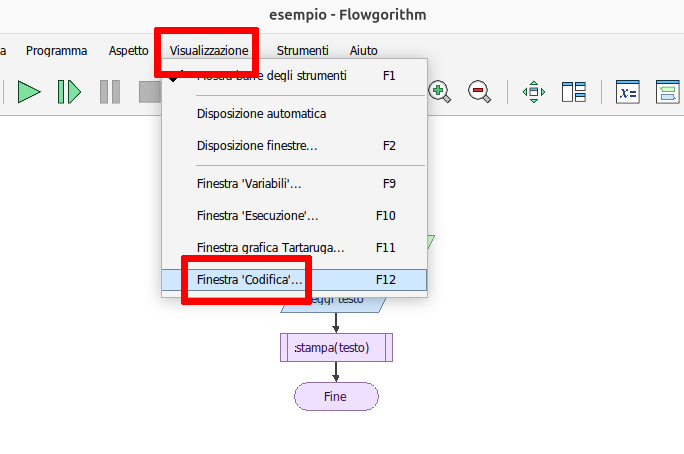
\includegraphics[width=\linewidth]{img/flowgorithm1.png}
                    \caption{{Screenshot di \href{www.flowgorithm.org}{Flowgorithm} 
                    modificato tramite \href{https://www.gimp.org/}{GIMP}}}
                \end{figure}}
                \only<2 | handout:2>{\begin{figure}
                    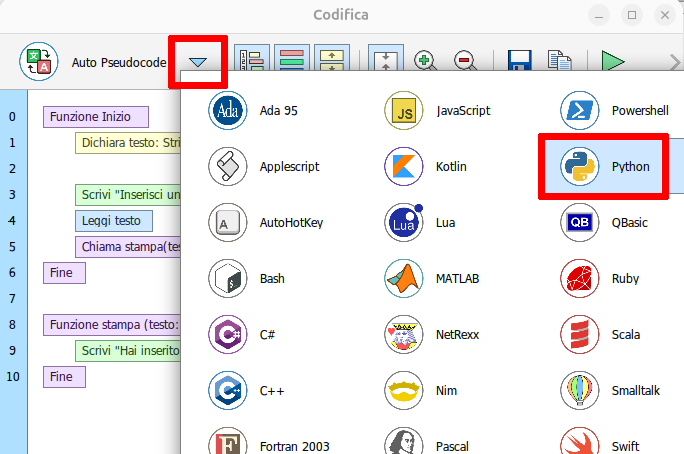
\includegraphics[width=\linewidth]{img/flowgorithm2.png}
                    \caption{{Screenshot di \href{www.flowgorithm.org}{Flowgorithm} 
                    modificato tramite \href{https://www.gimp.org/}{GIMP}}}
                \end{figure}}
                \only<3 | handout:3>{\begin{figure}
                    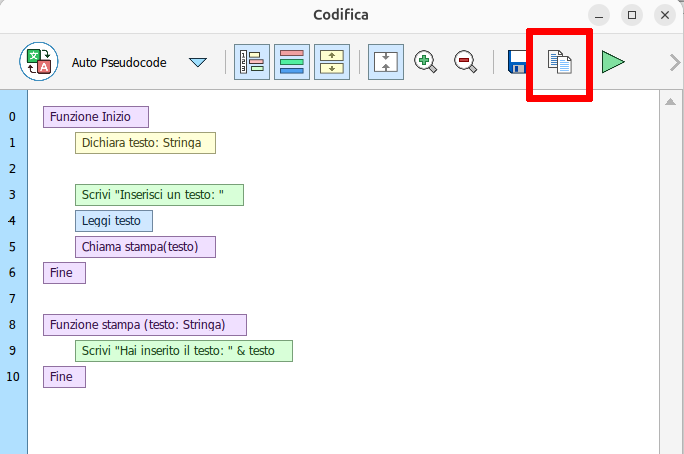
\includegraphics[width=\linewidth]{img/flowgorithm3.png}
                    \caption{{Screenshot di \href{www.flowgorithm.org}{Flowgorithm} 
                    modificato tramite \href{https://www.gimp.org/}{GIMP}}}
                \end{figure}}
            \end{figure}
    \end{columns}
\end{frame}

\section{TERZO PASSO: CREAZIONE DEL FILE .PY}

\begin{frame}{FROM FLOWGORITHM TO PYTHON}
    \begin{columns}
        \column{.5\textwidth}
            \begin{alertblock}{CREAZIONE DEL FILE .PY}
                \begin{minipage}{0.96\linewidth}
                    \justifying
                        \begin{itemize}
                            \item Apri Visual Studio Code e clicca su File $\rightarrow$ New File;
                            \pause
                            \item Salva il file con il nome del tuo progetto ed estensione .py sul Desktop;
                            \pause
                            \item Incolla il codice Python copiato da Flowgorithm all’interno del file .py;
                            \pause
                            \item Salva il file .py cliccando Ctrl + S (viene mostrata una X al posto di un cerchio).
                        \end{itemize}
                \end{minipage}
            \end{alertblock}
        \column{.5\textwidth}
            \begin{figure}
                \only<1 | handout:1>{\begin{figure}
                    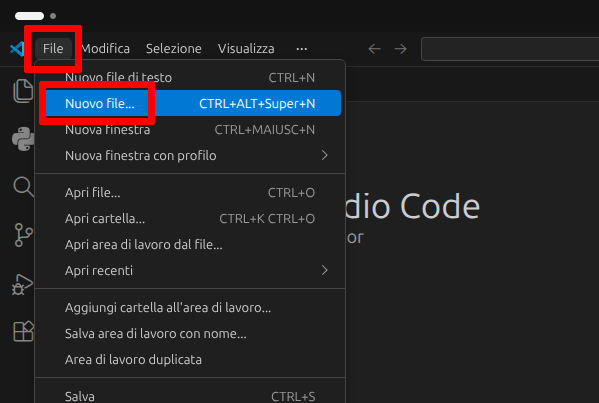
\includegraphics[width=\linewidth]{img/vscode1.png}
                    \caption{{Screenshot di \href{https://code.visualstudio.com/}{Visual Studio Code} 
                    modificato tramite \href{https://www.gimp.org/}{GIMP}}}
                \end{figure}}
                \only<2 | handout:2>{\begin{figure}
                    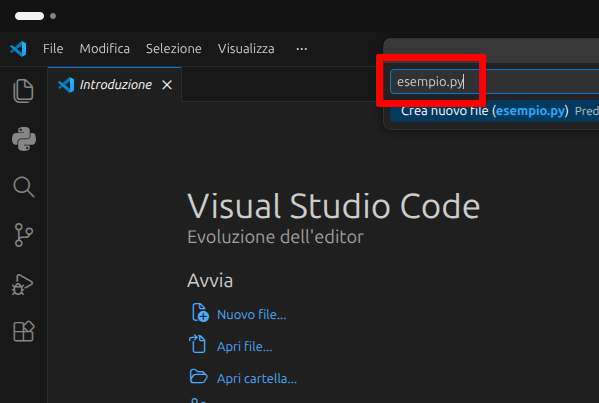
\includegraphics[width=\linewidth]{img/vscode2.png}
                    \caption{{Screenshot di \href{https://code.visualstudio.com/}{Visual Studio Code} 
                    modificato tramite \href{https://www.gimp.org/}{GIMP}}}
                \end{figure}}
                \only<3 | handout:3>{\begin{figure}
                    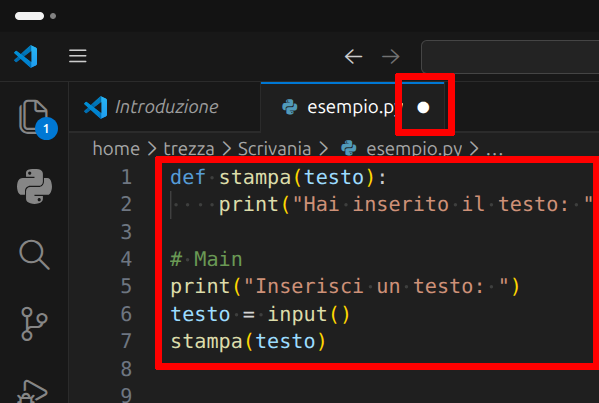
\includegraphics[width=\linewidth]{img/vscode3.png}
                    \caption{{Screenshot di \href{https://code.visualstudio.com/}{Visual Studio Code} 
                    modificato tramite \href{https://www.gimp.org/}{GIMP}}}
                \end{figure}}
                \only<4 | handout:4>{\begin{figure}
                    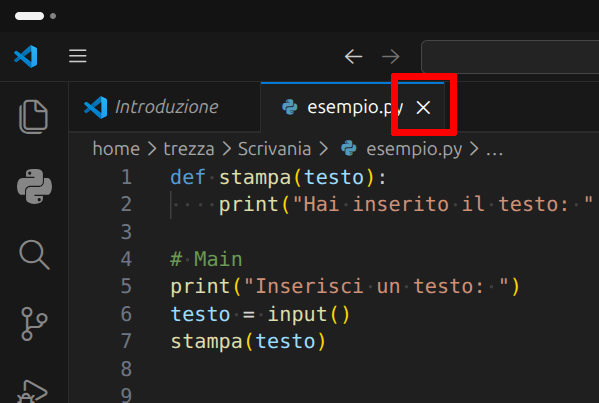
\includegraphics[width=\linewidth]{img/vscode4.png}
                    \caption{{Screenshot di \href{https://code.visualstudio.com/}{Visual Studio Code} 
                    modificato tramite \href{https://www.gimp.org/}{GIMP}}}                    
                \end{figure}}
            \end{figure}
    \end{columns}
\end{frame}

\section{QUARTO PASSO: HOW TO PLAY}

\begin{frame}{HOW TO PLAY}
    \begin{itemize}
        \justifying
        \item Apri il prompt dei comandi dal menu Start di Windows: \textbf{\textcolor{red}{CMD}};
        \pause
        \item Digita il comando \textbf{\textcolor{red}{cd desktop}} e premi Invio per accedere al desktop;
        \pause
        \item Digita il comando \textbf{\textcolor{red}{py}} seguito dal nome del file del tuo progetto compresa 
        l’estensione .py e premi Invio per iniziare a giocare, esempio: \textbf{\textcolor{red}{py esempio.py}}.
    \end{itemize}
\end{frame}

\end{document}